\documentclass[twoside]{book}

% Packages required by doxygen
\usepackage{fixltx2e}
\usepackage{calc}
\usepackage{doxygen}
\usepackage[export]{adjustbox} % also loads graphicx
\usepackage{graphicx}
\usepackage[utf8]{inputenc}
\usepackage{makeidx}
\usepackage{multicol}
\usepackage{multirow}
\PassOptionsToPackage{warn}{textcomp}
\usepackage{textcomp}
\usepackage[nointegrals]{wasysym}
\usepackage[table]{xcolor}

% Font selection
\usepackage[T1]{fontenc}
\usepackage[scaled=.90]{helvet}
\usepackage{courier}
\usepackage{amssymb}
\usepackage{sectsty}
\renewcommand{\familydefault}{\sfdefault}
\allsectionsfont{%
  \fontseries{bc}\selectfont%
  \color{darkgray}%
}
\renewcommand{\DoxyLabelFont}{%
  \fontseries{bc}\selectfont%
  \color{darkgray}%
}
\newcommand{\+}{\discretionary{\mbox{\scriptsize$\hookleftarrow$}}{}{}}

% Page & text layout
\usepackage{geometry}
\geometry{%
  a4paper,%
  top=2.5cm,%
  bottom=2.5cm,%
  left=2.5cm,%
  right=2.5cm%
}
\tolerance=750
\hfuzz=15pt
\hbadness=750
\setlength{\emergencystretch}{15pt}
\setlength{\parindent}{0cm}
\setlength{\parskip}{3ex plus 2ex minus 2ex}
\makeatletter
\renewcommand{\paragraph}{%
  \@startsection{paragraph}{4}{0ex}{-1.0ex}{1.0ex}{%
    \normalfont\normalsize\bfseries\SS@parafont%
  }%
}
\renewcommand{\subparagraph}{%
  \@startsection{subparagraph}{5}{0ex}{-1.0ex}{1.0ex}{%
    \normalfont\normalsize\bfseries\SS@subparafont%
  }%
}
\makeatother

% Headers & footers
\usepackage{fancyhdr}
\pagestyle{fancyplain}
\fancyhead[LE]{\fancyplain{}{\bfseries\thepage}}
\fancyhead[CE]{\fancyplain{}{}}
\fancyhead[RE]{\fancyplain{}{\bfseries\leftmark}}
\fancyhead[LO]{\fancyplain{}{\bfseries\rightmark}}
\fancyhead[CO]{\fancyplain{}{}}
\fancyhead[RO]{\fancyplain{}{\bfseries\thepage}}
\fancyfoot[LE]{\fancyplain{}{}}
\fancyfoot[CE]{\fancyplain{}{}}
\fancyfoot[RE]{\fancyplain{}{\bfseries\scriptsize Generated by Doxygen }}
\fancyfoot[LO]{\fancyplain{}{\bfseries\scriptsize Generated by Doxygen }}
\fancyfoot[CO]{\fancyplain{}{}}
\fancyfoot[RO]{\fancyplain{}{}}
\renewcommand{\footrulewidth}{0.4pt}
\renewcommand{\chaptermark}[1]{%
  \markboth{#1}{}%
}
\renewcommand{\sectionmark}[1]{%
  \markright{\thesection\ #1}%
}

% Indices & bibliography
\usepackage{natbib}
\usepackage[titles]{tocloft}
\setcounter{tocdepth}{3}
\setcounter{secnumdepth}{5}
\makeindex

% Hyperlinks (required, but should be loaded last)
\usepackage{ifpdf}
\ifpdf
  \usepackage[pdftex,pagebackref=true]{hyperref}
\else
  \usepackage[ps2pdf,pagebackref=true]{hyperref}
\fi
\hypersetup{%
  colorlinks=true,%
  linkcolor=blue,%
  citecolor=blue,%
  unicode%
}

% Custom commands
\newcommand{\clearemptydoublepage}{%
  \newpage{\pagestyle{empty}\cleardoublepage}%
}

\usepackage{caption}
\captionsetup{labelsep=space,justification=centering,font={bf},singlelinecheck=off,skip=4pt,position=top}

%===== C O N T E N T S =====

\begin{document}

% Titlepage & ToC
\hypersetup{pageanchor=false,
             bookmarksnumbered=true,
             pdfencoding=unicode
            }
\pagenumbering{alph}
\begin{titlepage}
\vspace*{7cm}
\begin{center}%
{\Large Entis }\\
\vspace*{1cm}
{\large Generated by Doxygen 1.8.13}\\
\end{center}
\end{titlepage}
\clearemptydoublepage
\pagenumbering{roman}
\tableofcontents
\clearemptydoublepage
\pagenumbering{arabic}
\hypersetup{pageanchor=true}

%--- Begin generated contents ---
\chapter{Module Index}
\section{Modules}
Here is a list of all modules\+:\begin{DoxyCompactList}
\item \contentsline{section}{General}{\pageref{group__General}}{}
\end{DoxyCompactList}

\chapter{Class Index}
\section{Class List}
Here are the classes, structs, unions and interfaces with brief descriptions\+:\begin{DoxyCompactList}
\item\contentsline{section}{\hyperlink{structentis__button__event}{entis\+\_\+button\+\_\+event} }{\pageref{structentis__button__event}}{}
\item\contentsline{section}{\hyperlink{structentis__circulate__event}{entis\+\_\+circulate\+\_\+event} }{\pageref{structentis__circulate__event}}{}
\item\contentsline{section}{\hyperlink{structentis__circulate__request__event}{entis\+\_\+circulate\+\_\+request\+\_\+event} }{\pageref{structentis__circulate__request__event}}{}
\item\contentsline{section}{\hyperlink{structentis__color}{entis\+\_\+color} }{\pageref{structentis__color}}{}
\item\contentsline{section}{\hyperlink{structentis__configure__event}{entis\+\_\+configure\+\_\+event} }{\pageref{structentis__configure__event}}{}
\item\contentsline{section}{\hyperlink{structentis__configure__request__event}{entis\+\_\+configure\+\_\+request\+\_\+event} }{\pageref{structentis__configure__request__event}}{}
\item\contentsline{section}{\hyperlink{structentis__create__event}{entis\+\_\+create\+\_\+event} }{\pageref{structentis__create__event}}{}
\item\contentsline{section}{\hyperlink{structentis__crossing__event}{entis\+\_\+crossing\+\_\+event} }{\pageref{structentis__crossing__event}}{}
\item\contentsline{section}{\hyperlink{structentis__destroy__event}{entis\+\_\+destroy\+\_\+event} }{\pageref{structentis__destroy__event}}{}
\item\contentsline{section}{\hyperlink{structentis__event}{entis\+\_\+event} }{\pageref{structentis__event}}{}
\item\contentsline{section}{\hyperlink{structentis__expose__event}{entis\+\_\+expose\+\_\+event} }{\pageref{structentis__expose__event}}{}
\item\contentsline{section}{\hyperlink{structentis__focus__event}{entis\+\_\+focus\+\_\+event} }{\pageref{structentis__focus__event}}{}
\item\contentsline{section}{\hyperlink{structentis__graphics__expose__event}{entis\+\_\+graphics\+\_\+expose\+\_\+event} }{\pageref{structentis__graphics__expose__event}}{}
\item\contentsline{section}{\hyperlink{structentis__gravity__event}{entis\+\_\+gravity\+\_\+event} }{\pageref{structentis__gravity__event}}{}
\item\contentsline{section}{\hyperlink{structentis__key__event}{entis\+\_\+key\+\_\+event} }{\pageref{structentis__key__event}}{}
\item\contentsline{section}{\hyperlink{structentis__map__event}{entis\+\_\+map\+\_\+event} }{\pageref{structentis__map__event}}{}
\item\contentsline{section}{\hyperlink{structentis__map__request__event}{entis\+\_\+map\+\_\+request\+\_\+event} }{\pageref{structentis__map__request__event}}{}
\item\contentsline{section}{\hyperlink{structentis__mapping__event}{entis\+\_\+mapping\+\_\+event} }{\pageref{structentis__mapping__event}}{}
\item\contentsline{section}{\hyperlink{structentis__motion__event}{entis\+\_\+motion\+\_\+event} }{\pageref{structentis__motion__event}}{}
\item\contentsline{section}{\hyperlink{structentis__no__expose__event}{entis\+\_\+no\+\_\+expose\+\_\+event} }{\pageref{structentis__no__expose__event}}{}
\item\contentsline{section}{\hyperlink{structentis__palette}{entis\+\_\+palette} }{\pageref{structentis__palette}}{}
\item\contentsline{section}{\hyperlink{structentis__property__event}{entis\+\_\+property\+\_\+event} }{\pageref{structentis__property__event}}{}
\item\contentsline{section}{\hyperlink{structentis__reparent__event}{entis\+\_\+reparent\+\_\+event} }{\pageref{structentis__reparent__event}}{}
\item\contentsline{section}{\hyperlink{structentis__resize__event}{entis\+\_\+resize\+\_\+event} }{\pageref{structentis__resize__event}}{}
\item\contentsline{section}{\hyperlink{structentis__selection__clear__event}{entis\+\_\+selection\+\_\+clear\+\_\+event} }{\pageref{structentis__selection__clear__event}}{}
\item\contentsline{section}{\hyperlink{structentis__selection__event}{entis\+\_\+selection\+\_\+event} }{\pageref{structentis__selection__event}}{}
\item\contentsline{section}{\hyperlink{structentis__selection__request__event}{entis\+\_\+selection\+\_\+request\+\_\+event} }{\pageref{structentis__selection__request__event}}{}
\item\contentsline{section}{\hyperlink{structentis__unmap__event}{entis\+\_\+unmap\+\_\+event} }{\pageref{structentis__unmap__event}}{}
\item\contentsline{section}{\hyperlink{structentis__visibility__event}{entis\+\_\+visibility\+\_\+event} }{\pageref{structentis__visibility__event}}{}
\end{DoxyCompactList}

\chapter{Module Documentation}
\hypertarget{group__General}{}\section{General}
\label{group__General}\index{General@{General}}
\subsection*{Functions}
\begin{DoxyCompactItemize}
\item 
void \hyperlink{group__General_ga9b2e862fe151d11a2f6564ff7c15688d}{entis\+\_\+init} (const char $\ast$title, unsigned int w, unsigned int h, uint32\+\_\+t value\+\_\+mask, void $\ast$value\+\_\+list)
\begin{DoxyCompactList}\small\item\em Initialize Entis library. \end{DoxyCompactList}\item 
void \hyperlink{group__General_ga12caa53e65fc497a009e460fff977b1c}{entis\+\_\+term} ()
\begin{DoxyCompactList}\small\item\em Terminates Entis library. \end{DoxyCompactList}\item 
bool \hyperlink{group__General_gada26de3271ef1aef670de8db756dea20}{entis\+\_\+connection\+\_\+valid} ()
\begin{DoxyCompactList}\small\item\em Checks if X\+CB connection is valid. \end{DoxyCompactList}\item 
void \hyperlink{group__General_gaae109a468964f275fa2deebd567b9aba}{entis\+\_\+flush} ()
\begin{DoxyCompactList}\small\item\em Flush X\+CB connections. \end{DoxyCompactList}\end{DoxyCompactItemize}


\subsection{Detailed Description}
General functions for support of the Entis library. 

\subsection{Function Documentation}
\mbox{\Hypertarget{group__General_gada26de3271ef1aef670de8db756dea20}\label{group__General_gada26de3271ef1aef670de8db756dea20}} 
\index{General@{General}!entis\+\_\+connection\+\_\+valid@{entis\+\_\+connection\+\_\+valid}}
\index{entis\+\_\+connection\+\_\+valid@{entis\+\_\+connection\+\_\+valid}!General@{General}}
\subsubsection{\texorpdfstring{entis\+\_\+connection\+\_\+valid()}{entis\_connection\_valid()}}
{\footnotesize\ttfamily bool entis\+\_\+connection\+\_\+valid (\begin{DoxyParamCaption}{ }\end{DoxyParamCaption})}



Checks if X\+CB connection is valid. 

Checks if the currently established X\+CB connection to the X server is valid.

\begin{DoxyReturn}{Returns}
{\ttfamily true} or {\ttfamily false}. 
\end{DoxyReturn}
\mbox{\Hypertarget{group__General_gaae109a468964f275fa2deebd567b9aba}\label{group__General_gaae109a468964f275fa2deebd567b9aba}} 
\index{General@{General}!entis\+\_\+flush@{entis\+\_\+flush}}
\index{entis\+\_\+flush@{entis\+\_\+flush}!General@{General}}
\subsubsection{\texorpdfstring{entis\+\_\+flush()}{entis\_flush()}}
{\footnotesize\ttfamily void entis\+\_\+flush (\begin{DoxyParamCaption}{ }\end{DoxyParamCaption})}



Flush X\+CB connections. 

Sends all requests to the X server. This must be done for any requests to be acted upon. \mbox{\Hypertarget{group__General_ga9b2e862fe151d11a2f6564ff7c15688d}\label{group__General_ga9b2e862fe151d11a2f6564ff7c15688d}} 
\index{General@{General}!entis\+\_\+init@{entis\+\_\+init}}
\index{entis\+\_\+init@{entis\+\_\+init}!General@{General}}
\subsubsection{\texorpdfstring{entis\+\_\+init()}{entis\_init()}}
{\footnotesize\ttfamily void entis\+\_\+init (\begin{DoxyParamCaption}\item[{const char $\ast$}]{title,  }\item[{unsigned int}]{w,  }\item[{unsigned int}]{h,  }\item[{uint32\+\_\+t}]{value\+\_\+mask,  }\item[{void $\ast$}]{value\+\_\+list }\end{DoxyParamCaption})}



Initialize Entis library. 

This {\bfseries must} be called before all other Entis calls. It generates the X\+CB connection to the X server, which is necessary for almost all functions present in the Entis library. Thus be sure to call this function before any other functions from Entis. It also generate a window with provided specifics.


\begin{DoxyParams}{Parameters}
{\em title} & Title of the window to generate. \\
\hline
{\em w} & Desired width of the window. \\
\hline
{\em h} & Desired height of the window. \\
\hline
{\em value\+\_\+mask} & Bit mask of values to alter the window. \\
\hline
{\em value\+\_\+list} & Values associated with provided bits in {\ttfamily value\+\_\+mask}. \\
\hline
\end{DoxyParams}
\mbox{\Hypertarget{group__General_ga12caa53e65fc497a009e460fff977b1c}\label{group__General_ga12caa53e65fc497a009e460fff977b1c}} 
\index{General@{General}!entis\+\_\+term@{entis\+\_\+term}}
\index{entis\+\_\+term@{entis\+\_\+term}!General@{General}}
\subsubsection{\texorpdfstring{entis\+\_\+term()}{entis\_term()}}
{\footnotesize\ttfamily void entis\+\_\+term (\begin{DoxyParamCaption}{ }\end{DoxyParamCaption})}



Terminates Entis library. 

This function {\bfseries must} be the final Entis function called. After it is called no other Entis function will work properly. It closes the X\+CB connection to the X server, which is necessary for almost all functions. This function will also close the generated window. 
\chapter{Class Documentation}
\hypertarget{structentis__button__event}{}\section{entis\+\_\+button\+\_\+event Struct Reference}
\label{structentis__button__event}\index{entis\+\_\+button\+\_\+event@{entis\+\_\+button\+\_\+event}}
\subsection*{Public Attributes}
\begin{DoxyCompactItemize}
\item 
\mbox{\Hypertarget{structentis__button__event_a65fb53f9490f5a61daa066615a237d2f}\label{structentis__button__event_a65fb53f9490f5a61daa066615a237d2f}} 
enum Event\+Type {\bfseries type}
\item 
\mbox{\Hypertarget{structentis__button__event_a3c1b558031ee2e1cd59bccb263735f15}\label{structentis__button__event_a3c1b558031ee2e1cd59bccb263735f15}} 
uint32\+\_\+t {\bfseries time}
\item 
\mbox{\Hypertarget{structentis__button__event_ad619f63529bda2ed6be07b6759355e4f}\label{structentis__button__event_ad619f63529bda2ed6be07b6759355e4f}} 
int16\+\_\+t {\bfseries x}
\item 
\mbox{\Hypertarget{structentis__button__event_aba7a0e9652a27aca0b4df5d8cab6e8e2}\label{structentis__button__event_aba7a0e9652a27aca0b4df5d8cab6e8e2}} 
int16\+\_\+t {\bfseries y}
\item 
\mbox{\Hypertarget{structentis__button__event_a102671036f50da00a4dcdf8a8af3d93b}\label{structentis__button__event_a102671036f50da00a4dcdf8a8af3d93b}} 
int16\+\_\+t {\bfseries root\+\_\+x}
\item 
\mbox{\Hypertarget{structentis__button__event_a2adbd682bf1448a5afe2caab9529d404}\label{structentis__button__event_a2adbd682bf1448a5afe2caab9529d404}} 
int16\+\_\+t {\bfseries root\+\_\+y}
\item 
\mbox{\Hypertarget{structentis__button__event_a2c678ba8ec98be1b0c048a234914fbe1}\label{structentis__button__event_a2c678ba8ec98be1b0c048a234914fbe1}} 
uint16\+\_\+t {\bfseries state}
\item 
\mbox{\Hypertarget{structentis__button__event_aa7889c0012ae8607f7d2d1f9a3e5c40c}\label{structentis__button__event_aa7889c0012ae8607f7d2d1f9a3e5c40c}} 
uint8\+\_\+t {\bfseries button}
\end{DoxyCompactItemize}


The documentation for this struct was generated from the following file\+:\begin{DoxyCompactItemize}
\item 
src/event.\+h\end{DoxyCompactItemize}

\hypertarget{structentis__circulate__event}{}\section{entis\+\_\+circulate\+\_\+event Struct Reference}
\label{structentis__circulate__event}\index{entis\+\_\+circulate\+\_\+event@{entis\+\_\+circulate\+\_\+event}}
\subsection*{Public Attributes}
\begin{DoxyCompactItemize}
\item 
\mbox{\Hypertarget{structentis__circulate__event_a1b5fb9a18d7d078b91bc2d84d1a79f4f}\label{structentis__circulate__event_a1b5fb9a18d7d078b91bc2d84d1a79f4f}} 
enum Event\+Type {\bfseries type}
\item 
\mbox{\Hypertarget{structentis__circulate__event_a734494f1caddbdea910629db8970038c}\label{structentis__circulate__event_a734494f1caddbdea910629db8970038c}} 
uint8\+\_\+t {\bfseries place}
\end{DoxyCompactItemize}


The documentation for this struct was generated from the following file\+:\begin{DoxyCompactItemize}
\item 
src/event.\+h\end{DoxyCompactItemize}

\hypertarget{structentis__circulate__request__event}{}\section{entis\+\_\+circulate\+\_\+request\+\_\+event Struct Reference}
\label{structentis__circulate__request__event}\index{entis\+\_\+circulate\+\_\+request\+\_\+event@{entis\+\_\+circulate\+\_\+request\+\_\+event}}
\subsection*{Public Attributes}
\begin{DoxyCompactItemize}
\item 
\mbox{\Hypertarget{structentis__circulate__request__event_a5f8cf7c548a4fbb33bf2a535e708cd18}\label{structentis__circulate__request__event_a5f8cf7c548a4fbb33bf2a535e708cd18}} 
enum Event\+Type {\bfseries type}
\item 
\mbox{\Hypertarget{structentis__circulate__request__event_ac1f66dff608ebfbb8a4210c9e50946b1}\label{structentis__circulate__request__event_ac1f66dff608ebfbb8a4210c9e50946b1}} 
uint8\+\_\+t {\bfseries place}
\end{DoxyCompactItemize}


The documentation for this struct was generated from the following file\+:\begin{DoxyCompactItemize}
\item 
src/event.\+h\end{DoxyCompactItemize}

\hypertarget{structentis__color}{}\section{entis\+\_\+color Struct Reference}
\label{structentis__color}\index{entis\+\_\+color@{entis\+\_\+color}}
\subsection*{Public Attributes}
\begin{DoxyCompactItemize}
\item 
\mbox{\Hypertarget{structentis__color_ac440b1c95bafd6783a7952fecb1145d4}\label{structentis__color_ac440b1c95bafd6783a7952fecb1145d4}} 
uint8\+\_\+t {\bfseries red}
\item 
\mbox{\Hypertarget{structentis__color_a68c2841cb3d90e05495b39efd454c081}\label{structentis__color_a68c2841cb3d90e05495b39efd454c081}} 
uint8\+\_\+t {\bfseries green}
\item 
\mbox{\Hypertarget{structentis__color_a3d303530e1f114708d5c93a799dec252}\label{structentis__color_a3d303530e1f114708d5c93a799dec252}} 
uint8\+\_\+t {\bfseries blue}
\end{DoxyCompactItemize}


The documentation for this struct was generated from the following file\+:\begin{DoxyCompactItemize}
\item 
src/color.\+h\end{DoxyCompactItemize}

\hypertarget{structentis__configure__event}{}\section{entis\+\_\+configure\+\_\+event Struct Reference}
\label{structentis__configure__event}\index{entis\+\_\+configure\+\_\+event@{entis\+\_\+configure\+\_\+event}}
\subsection*{Public Attributes}
\begin{DoxyCompactItemize}
\item 
\mbox{\Hypertarget{structentis__configure__event_ac77fc6d2b2d6f0e5635feea39d912365}\label{structentis__configure__event_ac77fc6d2b2d6f0e5635feea39d912365}} 
enum Event\+Type {\bfseries type}
\item 
\mbox{\Hypertarget{structentis__configure__event_afa4ca30b8d7d14dda2e1be88aaf20d47}\label{structentis__configure__event_afa4ca30b8d7d14dda2e1be88aaf20d47}} 
xcb\+\_\+window\+\_\+t {\bfseries window}
\item 
\mbox{\Hypertarget{structentis__configure__event_ab0d1d49096bffb326ca0877188096cdd}\label{structentis__configure__event_ab0d1d49096bffb326ca0877188096cdd}} 
uint16\+\_\+t {\bfseries x}
\item 
\mbox{\Hypertarget{structentis__configure__event_ab7bad3c677925aa3d374228bd5506ba8}\label{structentis__configure__event_ab7bad3c677925aa3d374228bd5506ba8}} 
uint16\+\_\+t {\bfseries y}
\item 
\mbox{\Hypertarget{structentis__configure__event_a87fc4bff891480c6df1085c5f7d9c66e}\label{structentis__configure__event_a87fc4bff891480c6df1085c5f7d9c66e}} 
uint16\+\_\+t {\bfseries width}
\item 
\mbox{\Hypertarget{structentis__configure__event_a5f6140e92335607d68a30cbdd34b76da}\label{structentis__configure__event_a5f6140e92335607d68a30cbdd34b76da}} 
uint16\+\_\+t {\bfseries height}
\item 
\mbox{\Hypertarget{structentis__configure__event_aa16b5e7b325b1fef479ac175eada817f}\label{structentis__configure__event_aa16b5e7b325b1fef479ac175eada817f}} 
uint16\+\_\+t {\bfseries border\+\_\+width}
\end{DoxyCompactItemize}


The documentation for this struct was generated from the following file\+:\begin{DoxyCompactItemize}
\item 
src/event.\+h\end{DoxyCompactItemize}

\hypertarget{structentis__configure__request__event}{}\section{entis\+\_\+configure\+\_\+request\+\_\+event Struct Reference}
\label{structentis__configure__request__event}\index{entis\+\_\+configure\+\_\+request\+\_\+event@{entis\+\_\+configure\+\_\+request\+\_\+event}}
\subsection*{Public Attributes}
\begin{DoxyCompactItemize}
\item 
\mbox{\Hypertarget{structentis__configure__request__event_a99dd5728f7024bcfcfe0401ecb669cab}\label{structentis__configure__request__event_a99dd5728f7024bcfcfe0401ecb669cab}} 
enum Event\+Type {\bfseries type}
\item 
\mbox{\Hypertarget{structentis__configure__request__event_abc9637b7b906ba07c8c311256b686da3}\label{structentis__configure__request__event_abc9637b7b906ba07c8c311256b686da3}} 
xcb\+\_\+window\+\_\+t {\bfseries window}
\item 
\mbox{\Hypertarget{structentis__configure__request__event_ac86b05866358d6af1782bb17d6ebc76e}\label{structentis__configure__request__event_ac86b05866358d6af1782bb17d6ebc76e}} 
xcb\+\_\+window\+\_\+t {\bfseries sibling}
\item 
\mbox{\Hypertarget{structentis__configure__request__event_a3ebc23fdd88e15cedad2cb679e7d9b0d}\label{structentis__configure__request__event_a3ebc23fdd88e15cedad2cb679e7d9b0d}} 
uint16\+\_\+t {\bfseries x}
\item 
\mbox{\Hypertarget{structentis__configure__request__event_a0d32060d16c74fe091d8ba90862a5ba8}\label{structentis__configure__request__event_a0d32060d16c74fe091d8ba90862a5ba8}} 
uint16\+\_\+t {\bfseries y}
\item 
\mbox{\Hypertarget{structentis__configure__request__event_a5cd0d955a96d811fd76a392a1f5e0bf6}\label{structentis__configure__request__event_a5cd0d955a96d811fd76a392a1f5e0bf6}} 
uint16\+\_\+t {\bfseries width}
\item 
\mbox{\Hypertarget{structentis__configure__request__event_aa7298d1bcd5164b7555973aad23cf162}\label{structentis__configure__request__event_aa7298d1bcd5164b7555973aad23cf162}} 
uint16\+\_\+t {\bfseries height}
\item 
\mbox{\Hypertarget{structentis__configure__request__event_a0046bb091233c06a271a80908fb74286}\label{structentis__configure__request__event_a0046bb091233c06a271a80908fb74286}} 
uint16\+\_\+t {\bfseries border\+\_\+width}
\item 
\mbox{\Hypertarget{structentis__configure__request__event_afc01d16f3606a824a2d6daf71995c49c}\label{structentis__configure__request__event_afc01d16f3606a824a2d6daf71995c49c}} 
uint16\+\_\+t {\bfseries value\+\_\+mask}
\end{DoxyCompactItemize}


The documentation for this struct was generated from the following file\+:\begin{DoxyCompactItemize}
\item 
src/event.\+h\end{DoxyCompactItemize}

\hypertarget{structentis__create__event}{}\section{entis\+\_\+create\+\_\+event Struct Reference}
\label{structentis__create__event}\index{entis\+\_\+create\+\_\+event@{entis\+\_\+create\+\_\+event}}
\subsection*{Public Attributes}
\begin{DoxyCompactItemize}
\item 
\mbox{\Hypertarget{structentis__create__event_a9d14d11bdf34f3f0adec7c9d05ae3d72}\label{structentis__create__event_a9d14d11bdf34f3f0adec7c9d05ae3d72}} 
enum Event\+Type {\bfseries type}
\item 
\mbox{\Hypertarget{structentis__create__event_a683c3709ae27e32fafa1b3ef0b5cedda}\label{structentis__create__event_a683c3709ae27e32fafa1b3ef0b5cedda}} 
uint16\+\_\+t {\bfseries x}
\item 
\mbox{\Hypertarget{structentis__create__event_aa917a9588ccd4e1b81172a88c8a31434}\label{structentis__create__event_aa917a9588ccd4e1b81172a88c8a31434}} 
uint16\+\_\+t {\bfseries y}
\item 
\mbox{\Hypertarget{structentis__create__event_adff2dc36834030fa2c1921376faee801}\label{structentis__create__event_adff2dc36834030fa2c1921376faee801}} 
uint16\+\_\+t {\bfseries width}
\item 
\mbox{\Hypertarget{structentis__create__event_a6b47465aec3646d05e948a692ec63c64}\label{structentis__create__event_a6b47465aec3646d05e948a692ec63c64}} 
uint16\+\_\+t {\bfseries height}
\item 
\mbox{\Hypertarget{structentis__create__event_aa678bab73d1108d0a05480f7c539b88e}\label{structentis__create__event_aa678bab73d1108d0a05480f7c539b88e}} 
uint16\+\_\+t {\bfseries border\+\_\+width}
\end{DoxyCompactItemize}


The documentation for this struct was generated from the following file\+:\begin{DoxyCompactItemize}
\item 
src/event.\+h\end{DoxyCompactItemize}

\hypertarget{structentis__crossing__event}{}\section{entis\+\_\+crossing\+\_\+event Struct Reference}
\label{structentis__crossing__event}\index{entis\+\_\+crossing\+\_\+event@{entis\+\_\+crossing\+\_\+event}}
\subsection*{Public Attributes}
\begin{DoxyCompactItemize}
\item 
\mbox{\Hypertarget{structentis__crossing__event_a0704f9ab8dcc7470a5d815858385d95b}\label{structentis__crossing__event_a0704f9ab8dcc7470a5d815858385d95b}} 
enum Event\+Type {\bfseries type}
\item 
\mbox{\Hypertarget{structentis__crossing__event_abff68169233c526bd9b97e5c230012f6}\label{structentis__crossing__event_abff68169233c526bd9b97e5c230012f6}} 
uint32\+\_\+t {\bfseries time}
\item 
\mbox{\Hypertarget{structentis__crossing__event_aa1ce0bafa36f51928e811ae8e67a2fc1}\label{structentis__crossing__event_aa1ce0bafa36f51928e811ae8e67a2fc1}} 
int16\+\_\+t {\bfseries x}
\item 
\mbox{\Hypertarget{structentis__crossing__event_a9d41070d2ee7fd0a3f7d124472008a3f}\label{structentis__crossing__event_a9d41070d2ee7fd0a3f7d124472008a3f}} 
int16\+\_\+t {\bfseries y}
\item 
\mbox{\Hypertarget{structentis__crossing__event_a37822adfb16aad7ffa24dc35dbd6cc63}\label{structentis__crossing__event_a37822adfb16aad7ffa24dc35dbd6cc63}} 
int16\+\_\+t {\bfseries root\+\_\+x}
\item 
\mbox{\Hypertarget{structentis__crossing__event_aba07aa05ed91f4c39122772fbb205198}\label{structentis__crossing__event_aba07aa05ed91f4c39122772fbb205198}} 
int16\+\_\+t {\bfseries root\+\_\+y}
\item 
\mbox{\Hypertarget{structentis__crossing__event_a51320a96afcfd1a43c8d5642b96f84a4}\label{structentis__crossing__event_a51320a96afcfd1a43c8d5642b96f84a4}} 
uint16\+\_\+t {\bfseries state}
\item 
\mbox{\Hypertarget{structentis__crossing__event_a4deebfaba719f0b90f83a7320b900cab}\label{structentis__crossing__event_a4deebfaba719f0b90f83a7320b900cab}} 
uint8\+\_\+t {\bfseries button}
\end{DoxyCompactItemize}


The documentation for this struct was generated from the following file\+:\begin{DoxyCompactItemize}
\item 
src/event.\+h\end{DoxyCompactItemize}

\hypertarget{structentis__destroy__event}{}\section{entis\+\_\+destroy\+\_\+event Struct Reference}
\label{structentis__destroy__event}\index{entis\+\_\+destroy\+\_\+event@{entis\+\_\+destroy\+\_\+event}}
\subsection*{Public Attributes}
\begin{DoxyCompactItemize}
\item 
\mbox{\Hypertarget{structentis__destroy__event_a4992cf39b7aea2ff76d0d7c84fd98316}\label{structentis__destroy__event_a4992cf39b7aea2ff76d0d7c84fd98316}} 
enum Event\+Type {\bfseries type}
\item 
\mbox{\Hypertarget{structentis__destroy__event_a151cbbeff38dcf3826ac946aecb274b1}\label{structentis__destroy__event_a151cbbeff38dcf3826ac946aecb274b1}} 
xcb\+\_\+window\+\_\+t {\bfseries window}
\end{DoxyCompactItemize}


The documentation for this struct was generated from the following file\+:\begin{DoxyCompactItemize}
\item 
src/event.\+h\end{DoxyCompactItemize}

\hypertarget{structentis__event}{}\section{entis\+\_\+event Struct Reference}
\label{structentis__event}\index{entis\+\_\+event@{entis\+\_\+event}}


Collaboration diagram for entis\+\_\+event\+:\nopagebreak
\begin{figure}[H]
\begin{center}
\leavevmode
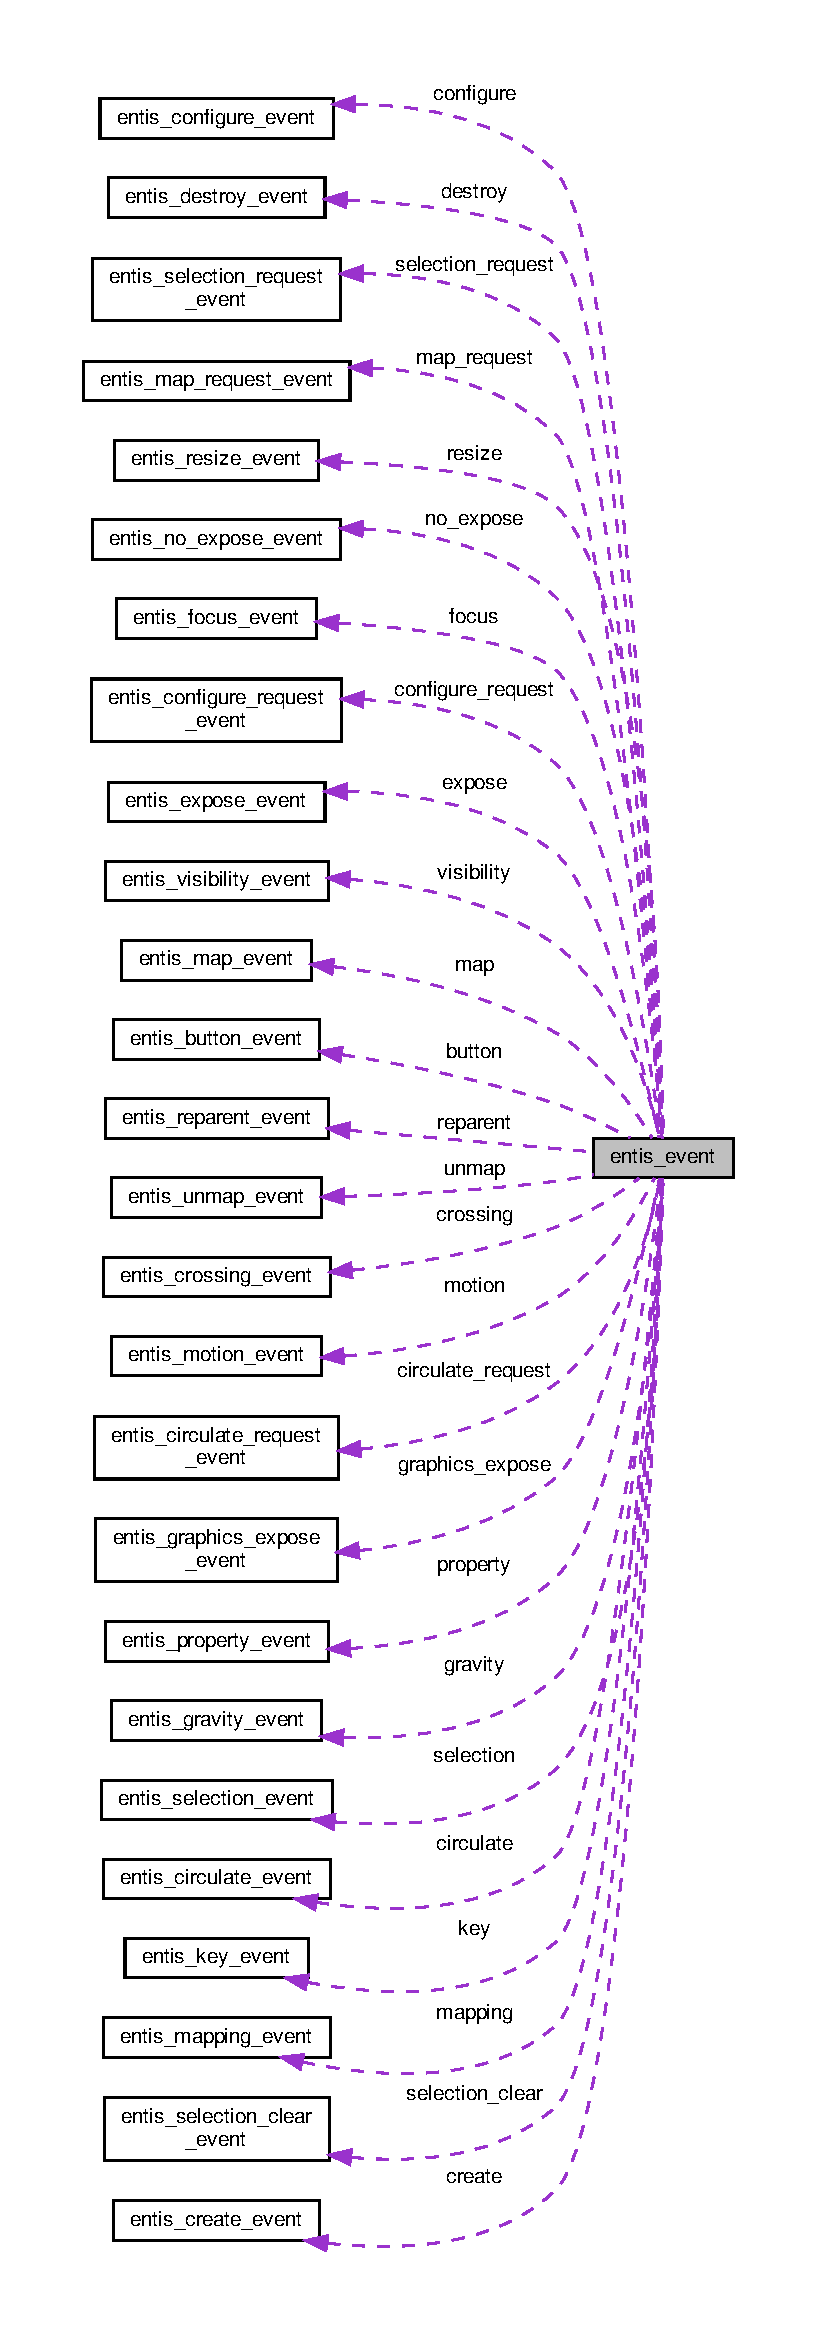
\includegraphics[height=550pt]{structentis__event__coll__graph}
\end{center}
\end{figure}
\subsection*{Public Attributes}
\begin{DoxyCompactItemize}
\item 
\mbox{\Hypertarget{structentis__event_aba10a3eaa7153c4dcf17e398ad01f0ae}\label{structentis__event_aba10a3eaa7153c4dcf17e398ad01f0ae}} 
enum Event\+Type {\bfseries type}
\item 
\mbox{\Hypertarget{structentis__event_a9ffe6b26ea904987bc30953503416975}\label{structentis__event_a9ffe6b26ea904987bc30953503416975}} 
\begin{tabbing}
xx\=xx\=xx\=xx\=xx\=xx\=xx\=xx\=xx\=\kill
union \{\\
\>\hyperlink{structentis__key__event}{entis\_key\_event} {\bfseries key}\\
\>\hyperlink{structentis__button__event}{entis\_button\_event} {\bfseries button}\\
\>\hyperlink{structentis__motion__event}{entis\_motion\_event} {\bfseries motion}\\
\>\hyperlink{structentis__crossing__event}{entis\_crossing\_event} {\bfseries crossing}\\
\>\hyperlink{structentis__focus__event}{entis\_focus\_event} {\bfseries focus}\\
\>\hyperlink{structentis__expose__event}{entis\_expose\_event} {\bfseries expose}\\
\>\hyperlink{structentis__graphics__expose__event}{entis\_graphics\_expose\_event} {\bfseries graphics\_expose}\\
\>\hyperlink{structentis__no__expose__event}{entis\_no\_expose\_event} {\bfseries no\_expose}\\
\>\hyperlink{structentis__visibility__event}{entis\_visibility\_event} {\bfseries visibility}\\
\>\hyperlink{structentis__create__event}{entis\_create\_event} {\bfseries create}\\
\>\hyperlink{structentis__destroy__event}{entis\_destroy\_event} {\bfseries destroy}\\
\>\hyperlink{structentis__unmap__event}{entis\_unmap\_event} {\bfseries unmap}\\
\>\hyperlink{structentis__map__event}{entis\_map\_event} {\bfseries map}\\
\>\hyperlink{structentis__map__request__event}{entis\_map\_request\_event} {\bfseries map\_request}\\
\>\hyperlink{structentis__reparent__event}{entis\_reparent\_event} {\bfseries reparent}\\
\>\hyperlink{structentis__configure__event}{entis\_configure\_event} {\bfseries configure}\\
\>\hyperlink{structentis__gravity__event}{entis\_gravity\_event} {\bfseries gravity}\\
\>\hyperlink{structentis__resize__event}{entis\_resize\_event} {\bfseries resize}\\
\>\hyperlink{structentis__configure__request__event}{entis\_configure\_request\_event} {\bfseries configure\_request}\\
\>\hyperlink{structentis__circulate__event}{entis\_circulate\_event} {\bfseries circulate}\\
\>\hyperlink{structentis__circulate__request__event}{entis\_circulate\_request\_event} {\bfseries circulate\_request}\\
\>\hyperlink{structentis__property__event}{entis\_property\_event} {\bfseries property}\\
\>\hyperlink{structentis__selection__event}{entis\_selection\_event} {\bfseries selection}\\
\>\hyperlink{structentis__selection__clear__event}{entis\_selection\_clear\_event} {\bfseries selection\_clear}\\
\>\hyperlink{structentis__selection__request__event}{entis\_selection\_request\_event} {\bfseries selection\_request}\\
\>\hyperlink{structentis__mapping__event}{entis\_mapping\_event} {\bfseries mapping}\\
\}; \\

\end{tabbing}\end{DoxyCompactItemize}


The documentation for this struct was generated from the following file\+:\begin{DoxyCompactItemize}
\item 
src/event.\+h\end{DoxyCompactItemize}

\hypertarget{structentis__expose__event}{}\section{entis\+\_\+expose\+\_\+event Struct Reference}
\label{structentis__expose__event}\index{entis\+\_\+expose\+\_\+event@{entis\+\_\+expose\+\_\+event}}
\subsection*{Public Attributes}
\begin{DoxyCompactItemize}
\item 
\mbox{\Hypertarget{structentis__expose__event_a6a17e29fd76012a767c3c08d2785dbbc}\label{structentis__expose__event_a6a17e29fd76012a767c3c08d2785dbbc}} 
enum Event\+Type {\bfseries type}
\item 
\mbox{\Hypertarget{structentis__expose__event_afd7b58a073125b967b3aa3fdf2747284}\label{structentis__expose__event_afd7b58a073125b967b3aa3fdf2747284}} 
uint16\+\_\+t {\bfseries x}
\item 
\mbox{\Hypertarget{structentis__expose__event_a5248e59eeb1496c28ae95397d57c8eb6}\label{structentis__expose__event_a5248e59eeb1496c28ae95397d57c8eb6}} 
uint16\+\_\+t {\bfseries y}
\item 
\mbox{\Hypertarget{structentis__expose__event_a23501fe4563c87552add40a608adf816}\label{structentis__expose__event_a23501fe4563c87552add40a608adf816}} 
uint16\+\_\+t {\bfseries width}
\item 
\mbox{\Hypertarget{structentis__expose__event_aa2120f5345c19d7569708deeb059b22d}\label{structentis__expose__event_aa2120f5345c19d7569708deeb059b22d}} 
uint16\+\_\+t {\bfseries height}
\item 
\mbox{\Hypertarget{structentis__expose__event_af1fa9b9400734a86f52fc78bb6fcd5f8}\label{structentis__expose__event_af1fa9b9400734a86f52fc78bb6fcd5f8}} 
uint16\+\_\+t {\bfseries count}
\end{DoxyCompactItemize}


The documentation for this struct was generated from the following file\+:\begin{DoxyCompactItemize}
\item 
src/event.\+h\end{DoxyCompactItemize}

\hypertarget{structentis__focus__event}{}\section{entis\+\_\+focus\+\_\+event Struct Reference}
\label{structentis__focus__event}\index{entis\+\_\+focus\+\_\+event@{entis\+\_\+focus\+\_\+event}}
\subsection*{Public Attributes}
\begin{DoxyCompactItemize}
\item 
\mbox{\Hypertarget{structentis__focus__event_aaf59df33e0bde67705f6429b8d3012d1}\label{structentis__focus__event_aaf59df33e0bde67705f6429b8d3012d1}} 
enum Event\+Type {\bfseries type}
\item 
\mbox{\Hypertarget{structentis__focus__event_ab194cc98d6854dee36222c0dad2daf32}\label{structentis__focus__event_ab194cc98d6854dee36222c0dad2daf32}} 
uint8\+\_\+t {\bfseries mode}
\item 
\mbox{\Hypertarget{structentis__focus__event_a944dc3ff091abaeaafe131c1cd8221ef}\label{structentis__focus__event_a944dc3ff091abaeaafe131c1cd8221ef}} 
uint8\+\_\+t {\bfseries detail}
\end{DoxyCompactItemize}


The documentation for this struct was generated from the following file\+:\begin{DoxyCompactItemize}
\item 
src/event.\+h\end{DoxyCompactItemize}

\hypertarget{structentis__graphics__expose__event}{}\section{entis\+\_\+graphics\+\_\+expose\+\_\+event Struct Reference}
\label{structentis__graphics__expose__event}\index{entis\+\_\+graphics\+\_\+expose\+\_\+event@{entis\+\_\+graphics\+\_\+expose\+\_\+event}}
\subsection*{Public Attributes}
\begin{DoxyCompactItemize}
\item 
\mbox{\Hypertarget{structentis__graphics__expose__event_a77150777a48328b11a58cdccb8aee3ad}\label{structentis__graphics__expose__event_a77150777a48328b11a58cdccb8aee3ad}} 
enum Event\+Type {\bfseries type}
\item 
\mbox{\Hypertarget{structentis__graphics__expose__event_a64d5a499a952784094cad1e42257deaa}\label{structentis__graphics__expose__event_a64d5a499a952784094cad1e42257deaa}} 
uint16\+\_\+t {\bfseries x}
\item 
\mbox{\Hypertarget{structentis__graphics__expose__event_a903f76814edb5e7328842dc11942cdd4}\label{structentis__graphics__expose__event_a903f76814edb5e7328842dc11942cdd4}} 
uint16\+\_\+t {\bfseries y}
\item 
\mbox{\Hypertarget{structentis__graphics__expose__event_a9ebe20f07f2cfa70c764d1594480dd60}\label{structentis__graphics__expose__event_a9ebe20f07f2cfa70c764d1594480dd60}} 
uint16\+\_\+t {\bfseries width}
\item 
\mbox{\Hypertarget{structentis__graphics__expose__event_a8533a874f95093b5e2de23f23caffe15}\label{structentis__graphics__expose__event_a8533a874f95093b5e2de23f23caffe15}} 
uint16\+\_\+t {\bfseries height}
\item 
\mbox{\Hypertarget{structentis__graphics__expose__event_a41abf701a0ed8f850ba713817fe76fdf}\label{structentis__graphics__expose__event_a41abf701a0ed8f850ba713817fe76fdf}} 
uint16\+\_\+t {\bfseries major}
\item 
\mbox{\Hypertarget{structentis__graphics__expose__event_a5333a312e5a43b7982634b31701302de}\label{structentis__graphics__expose__event_a5333a312e5a43b7982634b31701302de}} 
uint16\+\_\+t {\bfseries minor}
\item 
\mbox{\Hypertarget{structentis__graphics__expose__event_a852b1c2337c94837666e751a48f4f2b8}\label{structentis__graphics__expose__event_a852b1c2337c94837666e751a48f4f2b8}} 
uint16\+\_\+t {\bfseries count}
\end{DoxyCompactItemize}


The documentation for this struct was generated from the following file\+:\begin{DoxyCompactItemize}
\item 
src/event.\+h\end{DoxyCompactItemize}

\hypertarget{structentis__gravity__event}{}\section{entis\+\_\+gravity\+\_\+event Struct Reference}
\label{structentis__gravity__event}\index{entis\+\_\+gravity\+\_\+event@{entis\+\_\+gravity\+\_\+event}}
\subsection*{Public Attributes}
\begin{DoxyCompactItemize}
\item 
\mbox{\Hypertarget{structentis__gravity__event_a3c2d0cc34830a0100f6769db0575c97e}\label{structentis__gravity__event_a3c2d0cc34830a0100f6769db0575c97e}} 
enum Event\+Type {\bfseries type}
\item 
\mbox{\Hypertarget{structentis__gravity__event_ae45acbd1e3872c0afaf3792e6aba3728}\label{structentis__gravity__event_ae45acbd1e3872c0afaf3792e6aba3728}} 
xcb\+\_\+window\+\_\+t {\bfseries window}
\item 
\mbox{\Hypertarget{structentis__gravity__event_a9b7a307a6396a405770a68ca9c42d726}\label{structentis__gravity__event_a9b7a307a6396a405770a68ca9c42d726}} 
int16\+\_\+t {\bfseries x}
\item 
\mbox{\Hypertarget{structentis__gravity__event_a811e7ee3e2319d71a4e85862c6390fe8}\label{structentis__gravity__event_a811e7ee3e2319d71a4e85862c6390fe8}} 
int16\+\_\+t {\bfseries y}
\end{DoxyCompactItemize}


The documentation for this struct was generated from the following file\+:\begin{DoxyCompactItemize}
\item 
src/event.\+h\end{DoxyCompactItemize}

\hypertarget{structentis__key__event}{}\section{entis\+\_\+key\+\_\+event Struct Reference}
\label{structentis__key__event}\index{entis\+\_\+key\+\_\+event@{entis\+\_\+key\+\_\+event}}
\subsection*{Public Attributes}
\begin{DoxyCompactItemize}
\item 
\mbox{\Hypertarget{structentis__key__event_acf5927b79e4dc860edfbe3ca528bb561}\label{structentis__key__event_acf5927b79e4dc860edfbe3ca528bb561}} 
enum Event\+Type {\bfseries type}
\item 
\mbox{\Hypertarget{structentis__key__event_a50963a0de17809b9e6da95288a38eb6f}\label{structentis__key__event_a50963a0de17809b9e6da95288a38eb6f}} 
uint32\+\_\+t {\bfseries time}
\item 
\mbox{\Hypertarget{structentis__key__event_a506b13b95005a5674abd7d2f68d6fe7d}\label{structentis__key__event_a506b13b95005a5674abd7d2f68d6fe7d}} 
int16\+\_\+t {\bfseries x}
\item 
\mbox{\Hypertarget{structentis__key__event_afb1a26213a56db1c831bd068ba36eda4}\label{structentis__key__event_afb1a26213a56db1c831bd068ba36eda4}} 
int16\+\_\+t {\bfseries y}
\item 
\mbox{\Hypertarget{structentis__key__event_a6ab80ff4f3761ad52713d056b914c4ab}\label{structentis__key__event_a6ab80ff4f3761ad52713d056b914c4ab}} 
int16\+\_\+t {\bfseries root\+\_\+x}
\item 
\mbox{\Hypertarget{structentis__key__event_abe0d855028123011428db2790b3d00f3}\label{structentis__key__event_abe0d855028123011428db2790b3d00f3}} 
int16\+\_\+t {\bfseries root\+\_\+y}
\item 
\mbox{\Hypertarget{structentis__key__event_a9a68092a49f632fa014c9dd1e90a171a}\label{structentis__key__event_a9a68092a49f632fa014c9dd1e90a171a}} 
uint16\+\_\+t {\bfseries state}
\item 
\mbox{\Hypertarget{structentis__key__event_a2c2b3c23726c27aab6299264c22f6797}\label{structentis__key__event_a2c2b3c23726c27aab6299264c22f6797}} 
uint16\+\_\+t {\bfseries keycode}
\item 
\mbox{\Hypertarget{structentis__key__event_a04505239e7938b75f4ce3db9bec843f3}\label{structentis__key__event_a04505239e7938b75f4ce3db9bec843f3}} 
uint16\+\_\+t {\bfseries keysym}
\end{DoxyCompactItemize}


The documentation for this struct was generated from the following file\+:\begin{DoxyCompactItemize}
\item 
src/event.\+h\end{DoxyCompactItemize}

\hypertarget{structentis__map__event}{}\section{entis\+\_\+map\+\_\+event Struct Reference}
\label{structentis__map__event}\index{entis\+\_\+map\+\_\+event@{entis\+\_\+map\+\_\+event}}
\subsection*{Public Attributes}
\begin{DoxyCompactItemize}
\item 
\mbox{\Hypertarget{structentis__map__event_a567316ed6832e2c4d9a991493082a76d}\label{structentis__map__event_a567316ed6832e2c4d9a991493082a76d}} 
enum Event\+Type {\bfseries type}
\item 
\mbox{\Hypertarget{structentis__map__event_af31089ba27ac9e37a8c124b6e98848fb}\label{structentis__map__event_af31089ba27ac9e37a8c124b6e98848fb}} 
xcb\+\_\+window\+\_\+t {\bfseries window}
\end{DoxyCompactItemize}


The documentation for this struct was generated from the following file\+:\begin{DoxyCompactItemize}
\item 
src/event.\+h\end{DoxyCompactItemize}

\hypertarget{structentis__map__request__event}{}\section{entis\+\_\+map\+\_\+request\+\_\+event Struct Reference}
\label{structentis__map__request__event}\index{entis\+\_\+map\+\_\+request\+\_\+event@{entis\+\_\+map\+\_\+request\+\_\+event}}
\subsection*{Public Attributes}
\begin{DoxyCompactItemize}
\item 
\mbox{\Hypertarget{structentis__map__request__event_a4093dc4c8109300b32cdb8d2cb6b504e}\label{structentis__map__request__event_a4093dc4c8109300b32cdb8d2cb6b504e}} 
enum Event\+Type {\bfseries type}
\item 
\mbox{\Hypertarget{structentis__map__request__event_ab2f8ed98a3b181583107daccc199141f}\label{structentis__map__request__event_ab2f8ed98a3b181583107daccc199141f}} 
xcb\+\_\+window\+\_\+t {\bfseries parent}
\end{DoxyCompactItemize}


The documentation for this struct was generated from the following file\+:\begin{DoxyCompactItemize}
\item 
src/event.\+h\end{DoxyCompactItemize}

\hypertarget{structentis__mapping__event}{}\section{entis\+\_\+mapping\+\_\+event Struct Reference}
\label{structentis__mapping__event}\index{entis\+\_\+mapping\+\_\+event@{entis\+\_\+mapping\+\_\+event}}
\subsection*{Public Attributes}
\begin{DoxyCompactItemize}
\item 
\mbox{\Hypertarget{structentis__mapping__event_a6eb2526cdfb9e89ddd15617244ce44a9}\label{structentis__mapping__event_a6eb2526cdfb9e89ddd15617244ce44a9}} 
enum Event\+Type {\bfseries type}
\item 
\mbox{\Hypertarget{structentis__mapping__event_a5f506a2800f189cacc375a625340f979}\label{structentis__mapping__event_a5f506a2800f189cacc375a625340f979}} 
uint8\+\_\+t {\bfseries request}
\item 
\mbox{\Hypertarget{structentis__mapping__event_aa67bc39b4b1bdd6e45b1a4eae2a41a52}\label{structentis__mapping__event_aa67bc39b4b1bdd6e45b1a4eae2a41a52}} 
uint8\+\_\+t {\bfseries first\+\_\+keycode}
\item 
\mbox{\Hypertarget{structentis__mapping__event_a8d222c7d47f97bbcf48eef5a386ebcd0}\label{structentis__mapping__event_a8d222c7d47f97bbcf48eef5a386ebcd0}} 
uint8\+\_\+t {\bfseries count}
\end{DoxyCompactItemize}


The documentation for this struct was generated from the following file\+:\begin{DoxyCompactItemize}
\item 
src/event.\+h\end{DoxyCompactItemize}

\hypertarget{structentis__motion__event}{}\section{entis\+\_\+motion\+\_\+event Struct Reference}
\label{structentis__motion__event}\index{entis\+\_\+motion\+\_\+event@{entis\+\_\+motion\+\_\+event}}
\subsection*{Public Attributes}
\begin{DoxyCompactItemize}
\item 
\mbox{\Hypertarget{structentis__motion__event_aaea170b933103f0846b91d9a1bb267f8}\label{structentis__motion__event_aaea170b933103f0846b91d9a1bb267f8}} 
enum Event\+Type {\bfseries type}
\item 
\mbox{\Hypertarget{structentis__motion__event_a8821fe76a2f53de2e61688d73428978a}\label{structentis__motion__event_a8821fe76a2f53de2e61688d73428978a}} 
uint32\+\_\+t {\bfseries time}
\item 
\mbox{\Hypertarget{structentis__motion__event_a543febabcd244b05514b6a880543e464}\label{structentis__motion__event_a543febabcd244b05514b6a880543e464}} 
int16\+\_\+t {\bfseries x}
\item 
\mbox{\Hypertarget{structentis__motion__event_a05b9d879be66a647aa41af0382557da3}\label{structentis__motion__event_a05b9d879be66a647aa41af0382557da3}} 
int16\+\_\+t {\bfseries y}
\item 
\mbox{\Hypertarget{structentis__motion__event_af7f8bfe48c36677cab924cbaa8672b4f}\label{structentis__motion__event_af7f8bfe48c36677cab924cbaa8672b4f}} 
int16\+\_\+t {\bfseries root\+\_\+x}
\item 
\mbox{\Hypertarget{structentis__motion__event_a48823230db1d43e51c791520eb88b794}\label{structentis__motion__event_a48823230db1d43e51c791520eb88b794}} 
int16\+\_\+t {\bfseries root\+\_\+y}
\item 
\mbox{\Hypertarget{structentis__motion__event_a093c1cd2b716bdb6e39625f05c372ef3}\label{structentis__motion__event_a093c1cd2b716bdb6e39625f05c372ef3}} 
uint16\+\_\+t {\bfseries state}
\item 
\mbox{\Hypertarget{structentis__motion__event_a2bef24cfdce6f3ed754de366ab94e31e}\label{structentis__motion__event_a2bef24cfdce6f3ed754de366ab94e31e}} 
uint8\+\_\+t {\bfseries detail}
\end{DoxyCompactItemize}


The documentation for this struct was generated from the following file\+:\begin{DoxyCompactItemize}
\item 
src/event.\+h\end{DoxyCompactItemize}

\hypertarget{structentis__no__expose__event}{}\section{entis\+\_\+no\+\_\+expose\+\_\+event Struct Reference}
\label{structentis__no__expose__event}\index{entis\+\_\+no\+\_\+expose\+\_\+event@{entis\+\_\+no\+\_\+expose\+\_\+event}}
\subsection*{Public Attributes}
\begin{DoxyCompactItemize}
\item 
\mbox{\Hypertarget{structentis__no__expose__event_ae97828a656b3c946522b40c755063a50}\label{structentis__no__expose__event_ae97828a656b3c946522b40c755063a50}} 
enum Event\+Type {\bfseries type}
\item 
\mbox{\Hypertarget{structentis__no__expose__event_a7de719a7057a1c3a1937d26c452d4abb}\label{structentis__no__expose__event_a7de719a7057a1c3a1937d26c452d4abb}} 
uint16\+\_\+t {\bfseries major}
\item 
\mbox{\Hypertarget{structentis__no__expose__event_aeea14ed19ef9e3f2e17aec8e879119bc}\label{structentis__no__expose__event_aeea14ed19ef9e3f2e17aec8e879119bc}} 
uint16\+\_\+t {\bfseries minor}
\end{DoxyCompactItemize}


The documentation for this struct was generated from the following file\+:\begin{DoxyCompactItemize}
\item 
src/event.\+h\end{DoxyCompactItemize}

\hypertarget{structentis__palette}{}\section{entis\+\_\+palette Struct Reference}
\label{structentis__palette}\index{entis\+\_\+palette@{entis\+\_\+palette}}


Collaboration diagram for entis\+\_\+palette\+:\nopagebreak
\begin{figure}[H]
\begin{center}
\leavevmode
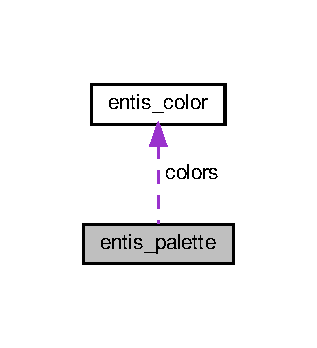
\includegraphics[width=152pt]{structentis__palette__coll__graph}
\end{center}
\end{figure}
\subsection*{Public Attributes}
\begin{DoxyCompactItemize}
\item 
\mbox{\Hypertarget{structentis__palette_a310189bf8fa2fd86b15cdd451a796588}\label{structentis__palette_a310189bf8fa2fd86b15cdd451a796588}} 
struct \hyperlink{structentis__color}{entis\+\_\+color} {\bfseries colors} \mbox{[}16\mbox{]}
\end{DoxyCompactItemize}


The documentation for this struct was generated from the following file\+:\begin{DoxyCompactItemize}
\item 
src/color.\+h\end{DoxyCompactItemize}

\hypertarget{structentis__property__event}{}\section{entis\+\_\+property\+\_\+event Struct Reference}
\label{structentis__property__event}\index{entis\+\_\+property\+\_\+event@{entis\+\_\+property\+\_\+event}}
\subsection*{Public Attributes}
\begin{DoxyCompactItemize}
\item 
\mbox{\Hypertarget{structentis__property__event_a5a827cdeeebde9bd07d030bc8587bdbf}\label{structentis__property__event_a5a827cdeeebde9bd07d030bc8587bdbf}} 
enum Event\+Type {\bfseries type}
\item 
\mbox{\Hypertarget{structentis__property__event_a5e75e2f9da15d72d7e7ebc519752ad31}\label{structentis__property__event_a5e75e2f9da15d72d7e7ebc519752ad31}} 
uint32\+\_\+t {\bfseries time}
\item 
\mbox{\Hypertarget{structentis__property__event_a18bac95d9c77019689226b9d0ebf04e7}\label{structentis__property__event_a18bac95d9c77019689226b9d0ebf04e7}} 
uint32\+\_\+t {\bfseries atom}
\item 
\mbox{\Hypertarget{structentis__property__event_a0c99abf727624f98a8b30361fe13caef}\label{structentis__property__event_a0c99abf727624f98a8b30361fe13caef}} 
uint8\+\_\+t {\bfseries state}
\end{DoxyCompactItemize}


The documentation for this struct was generated from the following file\+:\begin{DoxyCompactItemize}
\item 
src/event.\+h\end{DoxyCompactItemize}

\hypertarget{structentis__reparent__event}{}\section{entis\+\_\+reparent\+\_\+event Struct Reference}
\label{structentis__reparent__event}\index{entis\+\_\+reparent\+\_\+event@{entis\+\_\+reparent\+\_\+event}}
\subsection*{Public Attributes}
\begin{DoxyCompactItemize}
\item 
\mbox{\Hypertarget{structentis__reparent__event_ac5ff1ad76541f7e8357bd06c25f424ec}\label{structentis__reparent__event_ac5ff1ad76541f7e8357bd06c25f424ec}} 
enum Event\+Type {\bfseries type}
\item 
\mbox{\Hypertarget{structentis__reparent__event_a2359cdd927e3224e8af7cda378c25888}\label{structentis__reparent__event_a2359cdd927e3224e8af7cda378c25888}} 
xcb\+\_\+window\+\_\+t {\bfseries window}
\item 
\mbox{\Hypertarget{structentis__reparent__event_af06e126942bab6719175c004e500bb52}\label{structentis__reparent__event_af06e126942bab6719175c004e500bb52}} 
xcb\+\_\+window\+\_\+t {\bfseries parent}
\item 
\mbox{\Hypertarget{structentis__reparent__event_a64e0edbb3cd0cf3bb5254ba02fd11b6a}\label{structentis__reparent__event_a64e0edbb3cd0cf3bb5254ba02fd11b6a}} 
uint16\+\_\+t {\bfseries x}
\item 
\mbox{\Hypertarget{structentis__reparent__event_a00ef2aefb2de70b35ca53d716cd5bc17}\label{structentis__reparent__event_a00ef2aefb2de70b35ca53d716cd5bc17}} 
uint16\+\_\+t {\bfseries y}
\end{DoxyCompactItemize}


The documentation for this struct was generated from the following file\+:\begin{DoxyCompactItemize}
\item 
src/event.\+h\end{DoxyCompactItemize}

\hypertarget{structentis__resize__event}{}\section{entis\+\_\+resize\+\_\+event Struct Reference}
\label{structentis__resize__event}\index{entis\+\_\+resize\+\_\+event@{entis\+\_\+resize\+\_\+event}}
\subsection*{Public Attributes}
\begin{DoxyCompactItemize}
\item 
\mbox{\Hypertarget{structentis__resize__event_ad76e5ea08e83e2b03d0fde227737206f}\label{structentis__resize__event_ad76e5ea08e83e2b03d0fde227737206f}} 
enum Event\+Type {\bfseries type}
\item 
\mbox{\Hypertarget{structentis__resize__event_ab6b4a3e8b3480dc49377515d4d749de6}\label{structentis__resize__event_ab6b4a3e8b3480dc49377515d4d749de6}} 
xcb\+\_\+window\+\_\+t {\bfseries window}
\item 
\mbox{\Hypertarget{structentis__resize__event_a29360543a9a24b2c4910116d5c4ec197}\label{structentis__resize__event_a29360543a9a24b2c4910116d5c4ec197}} 
int16\+\_\+t {\bfseries width}
\item 
\mbox{\Hypertarget{structentis__resize__event_a9650e9c98e7b1ee90a93c3039d055de2}\label{structentis__resize__event_a9650e9c98e7b1ee90a93c3039d055de2}} 
int16\+\_\+t {\bfseries height}
\end{DoxyCompactItemize}


The documentation for this struct was generated from the following file\+:\begin{DoxyCompactItemize}
\item 
src/event.\+h\end{DoxyCompactItemize}

\hypertarget{structentis__selection__clear__event}{}\section{entis\+\_\+selection\+\_\+clear\+\_\+event Struct Reference}
\label{structentis__selection__clear__event}\index{entis\+\_\+selection\+\_\+clear\+\_\+event@{entis\+\_\+selection\+\_\+clear\+\_\+event}}
\subsection*{Public Attributes}
\begin{DoxyCompactItemize}
\item 
\mbox{\Hypertarget{structentis__selection__clear__event_a01326ac6bcfc5f3016acaf8809b085bf}\label{structentis__selection__clear__event_a01326ac6bcfc5f3016acaf8809b085bf}} 
enum Event\+Type {\bfseries type}
\item 
\mbox{\Hypertarget{structentis__selection__clear__event_ad0db2da6bacd76b164c6b22e61a4f5cf}\label{structentis__selection__clear__event_ad0db2da6bacd76b164c6b22e61a4f5cf}} 
uint32\+\_\+t {\bfseries selection}
\item 
\mbox{\Hypertarget{structentis__selection__clear__event_ab92a58eaa28b509dba7d539ae0ff8710}\label{structentis__selection__clear__event_ab92a58eaa28b509dba7d539ae0ff8710}} 
uint32\+\_\+t {\bfseries time}
\end{DoxyCompactItemize}


The documentation for this struct was generated from the following file\+:\begin{DoxyCompactItemize}
\item 
src/event.\+h\end{DoxyCompactItemize}

\hypertarget{structentis__selection__event}{}\section{entis\+\_\+selection\+\_\+event Struct Reference}
\label{structentis__selection__event}\index{entis\+\_\+selection\+\_\+event@{entis\+\_\+selection\+\_\+event}}
\subsection*{Public Attributes}
\begin{DoxyCompactItemize}
\item 
\mbox{\Hypertarget{structentis__selection__event_a4ea19c642e36c6e18c28fd62271503f9}\label{structentis__selection__event_a4ea19c642e36c6e18c28fd62271503f9}} 
enum Event\+Type {\bfseries type}
\item 
\mbox{\Hypertarget{structentis__selection__event_a84947ae6c0fd21f81d68be1622b4fd64}\label{structentis__selection__event_a84947ae6c0fd21f81d68be1622b4fd64}} 
xcb\+\_\+window\+\_\+t {\bfseries requestor}
\item 
\mbox{\Hypertarget{structentis__selection__event_a1a3a4a9427cd1ede59b33b480749e19a}\label{structentis__selection__event_a1a3a4a9427cd1ede59b33b480749e19a}} 
uint32\+\_\+t {\bfseries selection}
\item 
\mbox{\Hypertarget{structentis__selection__event_afbd962bddc653fd69d26d6980f53d662}\label{structentis__selection__event_afbd962bddc653fd69d26d6980f53d662}} 
uint32\+\_\+t {\bfseries target}
\item 
\mbox{\Hypertarget{structentis__selection__event_a21b47f52968ab2c08d10aa7ac55606ca}\label{structentis__selection__event_a21b47f52968ab2c08d10aa7ac55606ca}} 
uint32\+\_\+t {\bfseries property}
\item 
\mbox{\Hypertarget{structentis__selection__event_a1fe2e2039286aa15f71706ace6d48cc0}\label{structentis__selection__event_a1fe2e2039286aa15f71706ace6d48cc0}} 
uint32\+\_\+t {\bfseries time}
\end{DoxyCompactItemize}


The documentation for this struct was generated from the following file\+:\begin{DoxyCompactItemize}
\item 
src/event.\+h\end{DoxyCompactItemize}

\hypertarget{structentis__selection__request__event}{}\section{entis\+\_\+selection\+\_\+request\+\_\+event Struct Reference}
\label{structentis__selection__request__event}\index{entis\+\_\+selection\+\_\+request\+\_\+event@{entis\+\_\+selection\+\_\+request\+\_\+event}}
\subsection*{Public Attributes}
\begin{DoxyCompactItemize}
\item 
\mbox{\Hypertarget{structentis__selection__request__event_aee8904ac76db29ce9b0123bbd4d85b5c}\label{structentis__selection__request__event_aee8904ac76db29ce9b0123bbd4d85b5c}} 
enum Event\+Type {\bfseries type}
\item 
\mbox{\Hypertarget{structentis__selection__request__event_aaceb6c7f240b566ed54421ed896cd0a4}\label{structentis__selection__request__event_aaceb6c7f240b566ed54421ed896cd0a4}} 
xcb\+\_\+window\+\_\+t {\bfseries owner}
\item 
\mbox{\Hypertarget{structentis__selection__request__event_adc20713966136351b076a299bf7fb5b6}\label{structentis__selection__request__event_adc20713966136351b076a299bf7fb5b6}} 
xcb\+\_\+window\+\_\+t {\bfseries requestor}
\item 
\mbox{\Hypertarget{structentis__selection__request__event_a8cb4601af191b6011c3204f3a3fcfce4}\label{structentis__selection__request__event_a8cb4601af191b6011c3204f3a3fcfce4}} 
uint32\+\_\+t {\bfseries selection}
\item 
\mbox{\Hypertarget{structentis__selection__request__event_aae35872040ffbe27cc15d1240fc74c6d}\label{structentis__selection__request__event_aae35872040ffbe27cc15d1240fc74c6d}} 
uint32\+\_\+t {\bfseries target}
\item 
\mbox{\Hypertarget{structentis__selection__request__event_a8b1f33091c9d307fa4a43847f4670dfd}\label{structentis__selection__request__event_a8b1f33091c9d307fa4a43847f4670dfd}} 
uint32\+\_\+t {\bfseries property}
\item 
\mbox{\Hypertarget{structentis__selection__request__event_a4b4e856790b3f8f990a8da971ae33a1d}\label{structentis__selection__request__event_a4b4e856790b3f8f990a8da971ae33a1d}} 
uint32\+\_\+t {\bfseries time}
\end{DoxyCompactItemize}


The documentation for this struct was generated from the following file\+:\begin{DoxyCompactItemize}
\item 
src/event.\+h\end{DoxyCompactItemize}

\hypertarget{structentis__unmap__event}{}\section{entis\+\_\+unmap\+\_\+event Struct Reference}
\label{structentis__unmap__event}\index{entis\+\_\+unmap\+\_\+event@{entis\+\_\+unmap\+\_\+event}}
\subsection*{Public Attributes}
\begin{DoxyCompactItemize}
\item 
\mbox{\Hypertarget{structentis__unmap__event_ad564ac4108064d524226d414aedf52a8}\label{structentis__unmap__event_ad564ac4108064d524226d414aedf52a8}} 
enum Event\+Type {\bfseries type}
\item 
\mbox{\Hypertarget{structentis__unmap__event_ae19864ad8a3603dc17302e50f1cb14dd}\label{structentis__unmap__event_ae19864ad8a3603dc17302e50f1cb14dd}} 
xcb\+\_\+window\+\_\+t {\bfseries window}
\end{DoxyCompactItemize}


The documentation for this struct was generated from the following file\+:\begin{DoxyCompactItemize}
\item 
src/event.\+h\end{DoxyCompactItemize}

\hypertarget{structentis__visibility__event}{}\section{entis\+\_\+visibility\+\_\+event Struct Reference}
\label{structentis__visibility__event}\index{entis\+\_\+visibility\+\_\+event@{entis\+\_\+visibility\+\_\+event}}
\subsection*{Public Attributes}
\begin{DoxyCompactItemize}
\item 
\mbox{\Hypertarget{structentis__visibility__event_a24973762c7e625289fa844d530c92bb7}\label{structentis__visibility__event_a24973762c7e625289fa844d530c92bb7}} 
enum Event\+Type {\bfseries type}
\item 
\mbox{\Hypertarget{structentis__visibility__event_a6b96f2de6bdf0c114dc9583f387aecae}\label{structentis__visibility__event_a6b96f2de6bdf0c114dc9583f387aecae}} 
uint8\+\_\+t {\bfseries state}
\end{DoxyCompactItemize}


The documentation for this struct was generated from the following file\+:\begin{DoxyCompactItemize}
\item 
src/event.\+h\end{DoxyCompactItemize}

%--- End generated contents ---

% Index
\backmatter
\newpage
\phantomsection
\clearemptydoublepage
\addcontentsline{toc}{chapter}{Index}
\printindex

\end{document}
